\documentclass{standalone}
\usepackage{tikz}
\usetikzlibrary{patterns, positioning}
\usepackage[sfdefault]{ClearSans} %% option 'sfdefault' activates Clear Sans as the default text font
\usepackage[T1]{fontenc}

\begin{document}
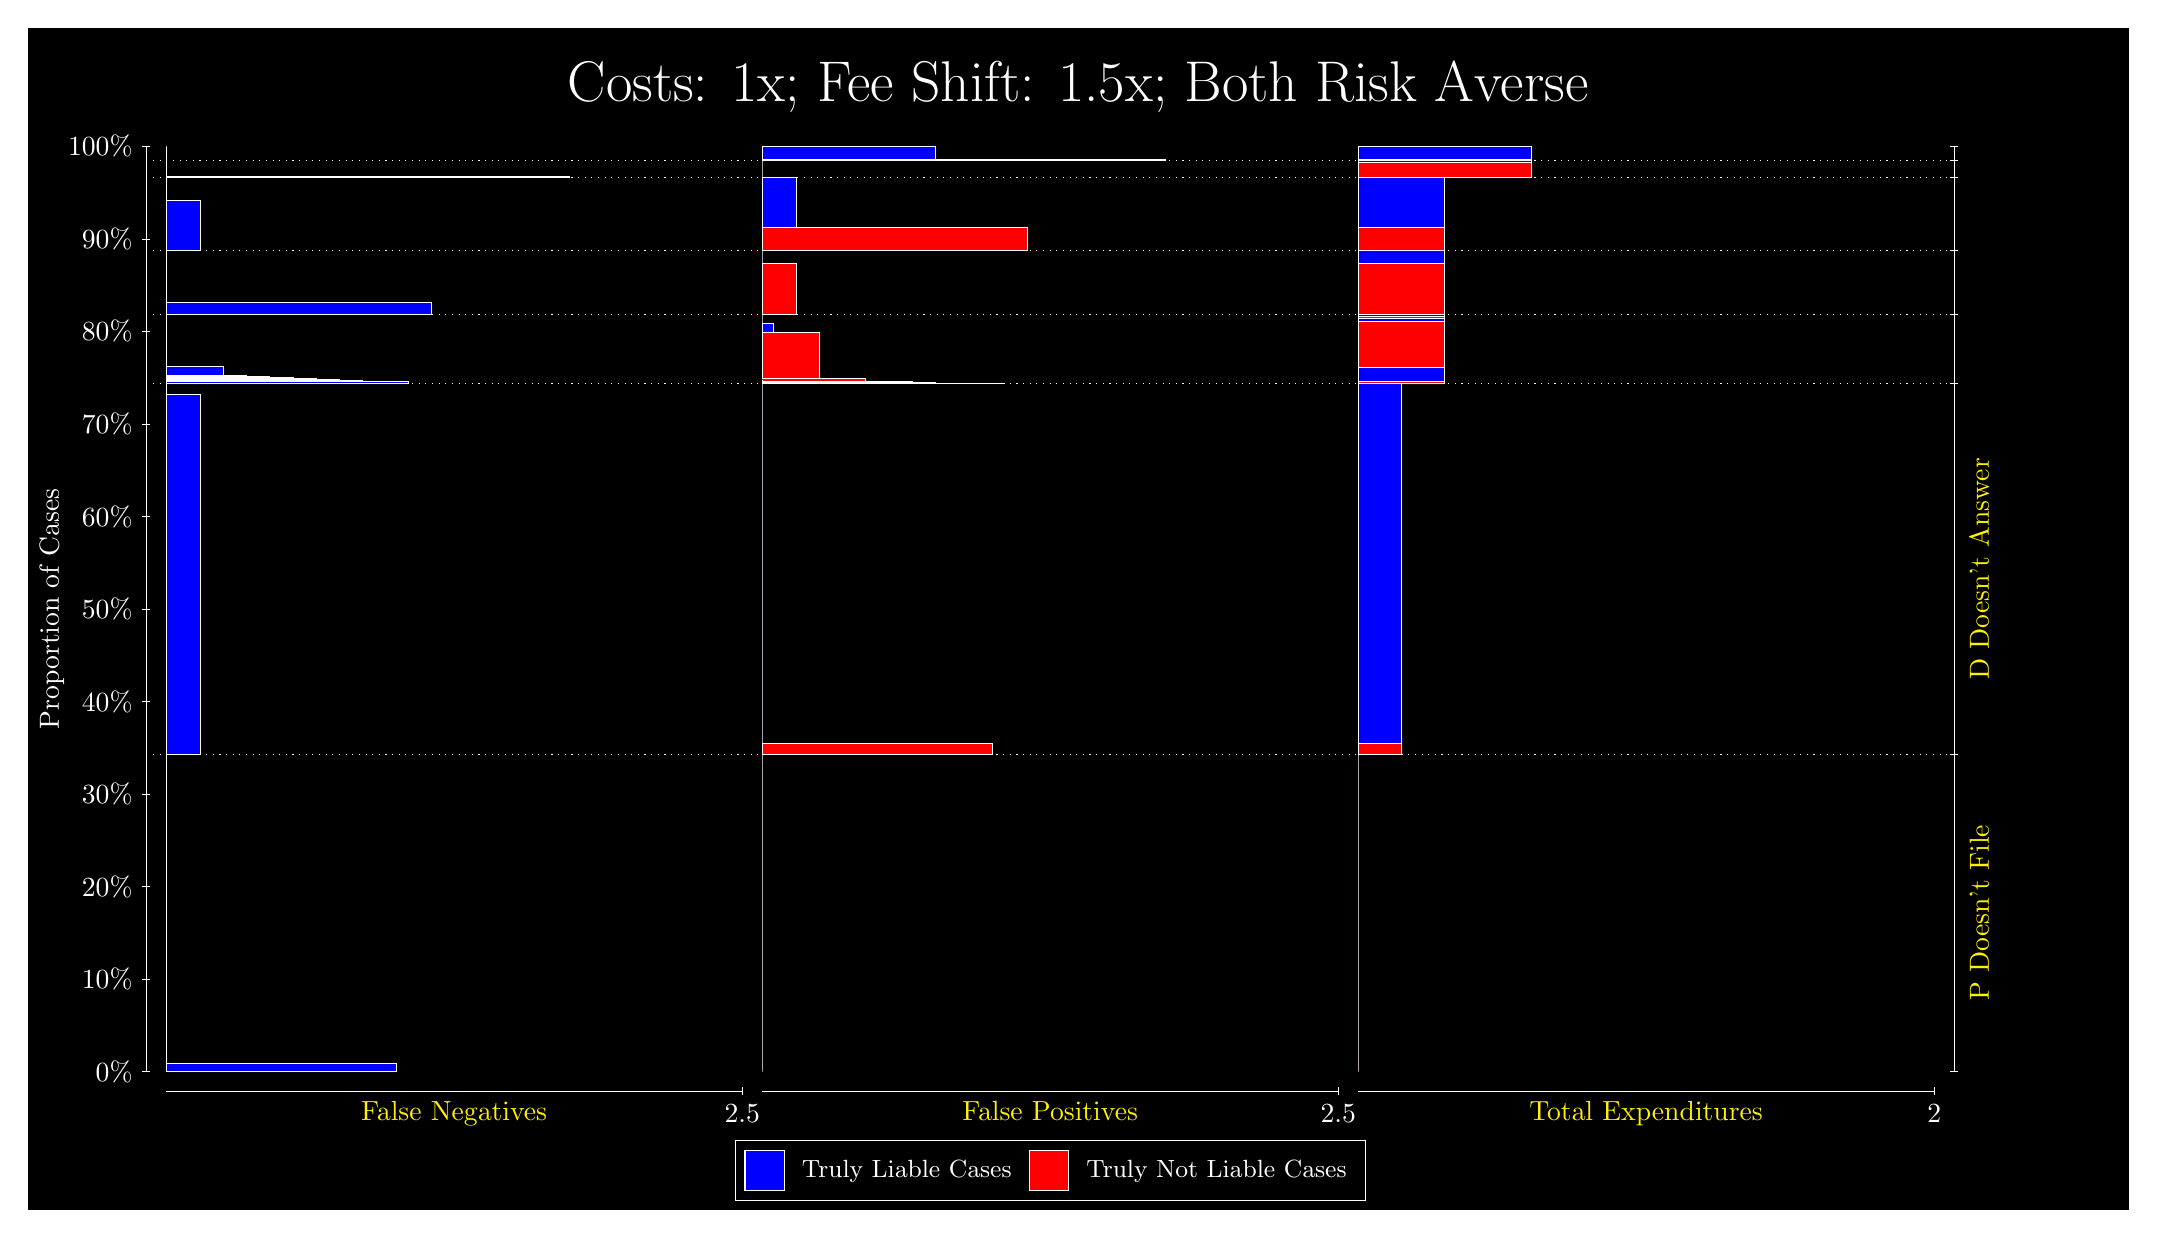
\begin{tikzpicture}
\draw[fill=black] (0,0) rectangle (26.667,15);
\draw[text=white] (0,13.5) rectangle (26.667,15) node[midway] {\huge Costs: 1x; Fee Shift: 1.5x; Both Risk Averse};
\draw[white, very thin] (1.5,1.75) -- (1.5,13.5);
\node[rotate=90, text=white, anchor=center] at (0.3, 7.625) {Proportion of Cases};
\draw[white, very thin] (1.45,1.75) -- (1.55,1.75);
\node[text=white, anchor=east] at (1.45, 1.75) {0\%};
\draw[white, very thin] (1.45,2.925) -- (1.55,2.925);
\node[text=white, anchor=east] at (1.45, 2.925) {10\%};
\draw[white, very thin] (1.45,4.1) -- (1.55,4.1);
\node[text=white, anchor=east] at (1.45, 4.1) {20\%};
\draw[white, very thin] (1.45,5.275) -- (1.55,5.275);
\node[text=white, anchor=east] at (1.45, 5.275) {30\%};
\draw[white, very thin] (1.45,6.45) -- (1.55,6.45);
\node[text=white, anchor=east] at (1.45, 6.45) {40\%};
\draw[white, very thin] (1.45,7.625) -- (1.55,7.625);
\node[text=white, anchor=east] at (1.45, 7.625) {50\%};
\draw[white, very thin] (1.45,8.8) -- (1.55,8.8);
\node[text=white, anchor=east] at (1.45, 8.8) {60\%};
\draw[white, very thin] (1.45,9.975) -- (1.55,9.975);
\node[text=white, anchor=east] at (1.45, 9.975) {70\%};
\draw[white, very thin] (1.45,11.15) -- (1.55,11.15);
\node[text=white, anchor=east] at (1.45, 11.15) {80\%};
\draw[white, very thin] (1.45,12.325) -- (1.55,12.325);
\node[text=white, anchor=east] at (1.45, 12.325) {90\%};
\draw[white, very thin] (1.45,13.5) -- (1.55,13.5);
\node[text=white, anchor=east] at (1.45, 13.5) {100\%};

\draw[white, very thin] (24.457,1.75) -- (24.457,13.5);
\draw[white, very thin] (24.407,1.75) -- (24.507,1.75);
\node[anchor=west] at (24.407, 1.75) {};
\draw[white, very thin] (24.407,5.7813) -- (24.507,5.7813);
\node[anchor=west] at (24.407, 5.7813) {};
\draw[white, very thin] (24.407,10.488) -- (24.507,10.488);
\node[anchor=west] at (24.407, 10.488) {};
\draw[white, very thin] (24.407,11.361) -- (24.507,11.361);
\node[anchor=west] at (24.407, 11.361) {};
\draw[white, very thin] (24.407,12.179) -- (24.507,12.179);
\node[anchor=west] at (24.407, 12.179) {};
\draw[white, very thin] (24.407,13.105) -- (24.507,13.105);
\node[anchor=west] at (24.407, 13.105) {};
\draw[white, very thin] (24.407,13.32) -- (24.507,13.32);
\node[anchor=west] at (24.407, 13.32) {};
\draw[white, very thin] (24.407,13.5) -- (24.507,13.5);
\node[anchor=west] at (24.407, 13.5) {};

\draw[white, very thin, fill=blue] (1.75,1.75) rectangle (4.6775,1.8566);
\draw[white, very thin, fill=red] (1.75,1.8566) rectangle (1.75,5.7813);
\draw[white, very thin, fill=blue] (1.75,5.7813) rectangle (2.1891,10.355);
\draw[white, very thin, fill=red] (1.75,10.355) rectangle (1.75,10.488);
\draw[white, very thin, fill=blue] (1.75,10.488) rectangle (4.8239,10.52);
\draw[white, very thin, fill=blue] (1.75,10.52) rectangle (4.5312,10.522);
\draw[white, very thin, fill=blue] (1.75,10.522) rectangle (4.2384,10.532);
\draw[white, very thin, fill=blue] (1.75,10.532) rectangle (3.9457,10.537);
\draw[white, very thin, fill=blue] (1.75,10.537) rectangle (3.6529,10.56);
\draw[white, very thin, fill=blue] (1.75,10.56) rectangle (3.3602,10.567);
\draw[white, very thin, fill=blue] (1.75,10.567) rectangle (3.0674,10.582);
\draw[white, very thin, fill=blue] (1.75,10.582) rectangle (2.7746,10.59);
\draw[white, very thin, fill=blue] (1.75,10.59) rectangle (2.4819,10.705);
\draw[white, very thin, fill=red] (1.75,10.705) rectangle (1.75,11.361);
\draw[white, very thin, fill=blue] (1.75,11.361) rectangle (5.1167,11.521);
\draw[white, very thin, fill=red] (1.75,11.521) rectangle (1.75,12.179);
\draw[white, very thin, fill=blue] (1.75,12.179) rectangle (2.1891,12.817);
\draw[white, very thin, fill=red] (1.75,12.817) rectangle (1.75,13.105);
\draw[white, very thin, fill=blue] (1.75,13.105) rectangle (6.8732,13.121);
\draw[white, very thin, fill=red] (1.75,13.121) rectangle (1.75,13.32);
\draw[white, very thin, fill=red] (1.75,13.32) rectangle (1.75,13.339);
\draw[white, very thin, fill=blue] (1.75,13.339) rectangle (1.75,13.5);
\draw[white, very thin, fill=red] (9.3189,1.75) rectangle (9.3189,5.6747);
\draw[white, very thin, fill=blue] (9.3189,5.6747) rectangle (9.3189,5.7813);
\draw[white, very thin, fill=red] (9.3189,5.7813) rectangle (12.246,5.9138);
\draw[white, very thin, fill=blue] (9.3189,5.9138) rectangle (9.3189,10.488);
\draw[white, very thin, fill=red] (9.3189,10.488) rectangle (12.393,10.492);
\draw[white, very thin, fill=red] (9.3189,10.492) rectangle (12.1,10.493);
\draw[white, very thin, fill=red] (9.3189,10.493) rectangle (11.807,10.496);
\draw[white, very thin, fill=red] (9.3189,10.496) rectangle (11.515,10.498);
\draw[white, very thin, fill=red] (9.3189,10.498) rectangle (11.222,10.516);
\draw[white, very thin, fill=red] (9.3189,10.516) rectangle (10.929,10.519);
\draw[white, very thin, fill=red] (9.3189,10.519) rectangle (10.929,10.521);
\draw[white, very thin, fill=red] (9.3189,10.521) rectangle (10.636,10.548);
\draw[white, very thin, fill=red] (9.3189,10.548) rectangle (10.344,10.549);
\draw[white, very thin, fill=red] (9.3189,10.549) rectangle (10.051,11.143);
\draw[white, very thin, fill=blue] (9.3189,11.143) rectangle (9.4652,11.258);
\draw[white, very thin, fill=blue] (9.3189,11.258) rectangle (9.3189,11.361);
\draw[white, very thin, fill=red] (9.3189,11.361) rectangle (9.758,12.018);
\draw[white, very thin, fill=blue] (9.3189,12.018) rectangle (9.3189,12.179);
\draw[white, very thin, fill=red] (9.3189,12.179) rectangle (12.686,12.466);
\draw[white, very thin, fill=blue] (9.3189,12.466) rectangle (9.758,13.105);
\draw[white, very thin, fill=red] (9.3189,13.105) rectangle (9.3189,13.303);
\draw[white, very thin, fill=blue] (9.3189,13.303) rectangle (9.3189,13.32);
\draw[white, very thin, fill=red] (9.3189,13.32) rectangle (14.442,13.339);
\draw[white, very thin, fill=blue] (9.3189,13.339) rectangle (11.515,13.5);
\draw[white, very thin, fill=red] (16.888,1.75) rectangle (16.888,5.6747);
\draw[white, very thin, fill=blue] (16.888,5.6747) rectangle (16.888,5.7813);
\draw[white, very thin, fill=red] (16.888,5.7813) rectangle (17.437,5.9138);
\draw[white, very thin, fill=blue] (16.888,5.9138) rectangle (17.437,10.488);
\draw[white, very thin, fill=red] (16.888,10.488) rectangle (17.986,10.519);
\draw[white, very thin, fill=blue] (16.888,10.519) rectangle (17.986,10.691);
\draw[white, very thin, fill=red] (16.888,10.691) rectangle (17.986,11.284);
\draw[white, very thin, fill=blue] (16.888,11.284) rectangle (17.986,11.316);
\draw[white, very thin, fill=red] (16.888,11.316) rectangle (17.986,11.346);
\draw[white, very thin, fill=blue] (16.888,11.346) rectangle (17.986,11.361);
\draw[white, very thin, fill=red] (16.888,11.361) rectangle (17.986,12.018);
\draw[white, very thin, fill=blue] (16.888,12.018) rectangle (17.986,12.179);
\draw[white, very thin, fill=red] (16.888,12.179) rectangle (17.986,12.466);
\draw[white, very thin, fill=blue] (16.888,12.466) rectangle (17.986,13.105);
\draw[white, very thin, fill=red] (16.888,13.105) rectangle (19.083,13.303);
\draw[white, very thin, fill=blue] (16.888,13.303) rectangle (19.083,13.32);
\draw[white, very thin, fill=red] (16.888,13.32) rectangle (19.083,13.339);
\draw[white, very thin, fill=blue] (16.888,13.339) rectangle (19.083,13.5);
\draw[white, dotted] (1.5,5.7813) -- (24.457,5.7813);
\draw[white, dotted] (1.5,10.488) -- (24.457,10.488);
\draw[white, dotted] (1.5,11.361) -- (24.457,11.361);
\draw[white, dotted] (1.5,12.179) -- (24.457,12.179);
\draw[white, dotted] (1.5,13.105) -- (24.457,13.105);
\draw[white, dotted] (1.5,13.32) -- (24.457,13.32);
\draw[white, very thin] (1.75,1.5) -- (9.0689,1.5);
\node[text=yellow, anchor=north] at (5.4094, 1.5) {False Negatives};
\draw[white, very thin] (9.0689,1.45) -- (9.0689,1.55);
\node[text=white, anchor=north] at (9.0689, 1.45) {2.5};

\draw[white, very thin] (9.3189,1.5) -- (16.638,1.5);
\node[text=yellow, anchor=north] at (12.978, 1.5) {False Positives};
\draw[white, very thin] (16.638,1.45) -- (16.638,1.55);
\node[text=white, anchor=north] at (16.638, 1.45) {2.5};

\draw[white, very thin] (16.888,1.5) -- (24.207,1.5);
\node[text=yellow, anchor=north] at (20.547, 1.5) {Total Expenditures};
\draw[white, very thin] (24.207,1.45) -- (24.207,1.55);
\node[text=white, anchor=north] at (24.207, 1.45) {2};

\node[text=yellow, centered, rotate=90] at (24.777, 3.7656) {P Doesn't File};
\node[text=yellow, centered, rotate=90] at (24.777, 8.1344) {D Doesn't Answer};






\draw (12.978300999999998,1.5) node[draw=none] (baseCoordinate) {};
\begin{scope}[align=center]
        \matrix[scale=0.5, draw=white, below=0.5cm of baseCoordinate, nodes={draw}, column sep=0.1cm]{
            \node[rectangle, draw, minimum width=0.5cm, minimum height=0.5cm, fill=blue] {}; &
            \node[draw=none, font=\small, text=white] (B) {Truly Liable Cases}; &
            \node[rectangle, draw, minimum width=0.5cm, minimum height=0.5cm, fill=red] {}; &
            \node[draw=none, font=\small, text=white] (B) {Truly Not Liable Cases}; \\
            };
\end{scope}

\end{tikzpicture}
\end{document}